\documentclass[12pt,a4paper]{article}
\usepackage[utf8]{inputenc}
\usepackage[T1]{fontenc}
\usepackage[english]{babel}
\usepackage{lmodern}
\usepackage{csquotes}
\usepackage{amsmath}
\usepackage{amssymb}
\usepackage{physics}
\usepackage{geometry}
\usepackage{tocloft}
\usepackage{xcolor}
\usepackage{graphicx,tikz,pgfplots}
\pgfplotsset{compat=1.18}
\usepackage{booktabs}
\usepackage{siunitx}
\usepackage{amsthm}
\usepackage[colorlinks=true, linkcolor=blue, citecolor=blue, urlcolor=blue]{hyperref}
\usepackage{cleveref}

\geometry{a4paper, margin=2cm}

\renewcommand{\cftsecfont}{\color{blue}}
\renewcommand{\cftsubsecfont}{\color{blue}}
\renewcommand{\cftsecpagefont}{\color{blue}}
\renewcommand{\cftsubsecpagefont}{\color{blue}}
\setlength{\cftsecindent}{1cm}
\setlength{\cftsubsecindent}{2cm}

\newcommand{\Tfield}{T(x)}

\newtheorem{theorem}{Theorem}[section]
\newtheorem{proposition}[theorem]{Proposition}

\title{Dynamic Mass of Photons and Its Implications for Nonlocality}
\author{Johann Pascher}
\date{March 25, 2025}

\begin{document}
	
	\maketitle
	
	\begin{abstract}
		This work explores the consequences of a dynamic, frequency-dependent mass for photons within various time models in quantum mechanics. By assigning \(m_\gamma = \omega\) in natural units, an energy-dependent time is introduced, impacting nonlocality and causality. The theory is supported by experimental predictions.
	\end{abstract}
	
	\tableofcontents
	\newpage
	
	\section{Introduction}
	This work examines the implications of a dynamic, frequency-dependent mass for photons within different quantum mechanical time models \cite{pascher1}.
	
	\section{Natural Units as a Foundation}
	\subsection{Definition of Natural Units}
	\begin{theorem}[Natural Units]
		With \(\hbar = c = G = 1\):
		\begin{align}
			[L] &= [E^{-1}] \\
			[T] &= [E^{-1}] \\
			[M] &= [E]
		\end{align}
	\end{theorem}
	
	\subsection{Significance for Mass-Energy Equivalence}
	\begin{equation}
		m_\gamma = \omega
	\end{equation}
	
	\section{Time Models in Quantum Mechanics}
	\subsection{Limitations of the Standard Model}
	\begin{equation}
		i\hbar\frac{\partial\psi}{\partial t} = H\psi
	\end{equation}
	
	\subsection{The T0 Model with Absolute Time}
	\begin{equation}
		E = \frac{\hbar}{T_0}
	\end{equation}
	
	\subsection{The Intrinsic Time Model}
	\begin{equation}
		\Tfield = \frac{\hbar}{mc^2}
	\end{equation}
	
	\subsection{Extension for Photons}
	\begin{equation}
		\Tfield = \frac{1}{E}
	\end{equation}
	
	\section{Unification of Models}
	\begin{equation}
		\Tfield = \frac{1}{\max(m, E)}
	\end{equation}
	
	\section{Implications for Nonlocality and Entanglement}
	\subsection{Energy-Dependent Correlations}
	\begin{itemize}
		\item Delay: \(\left|\frac{1}{E_1} - \frac{1}{E_2}\right|\)
	\end{itemize}
	
	\begin{figure}[h]
		\centering
		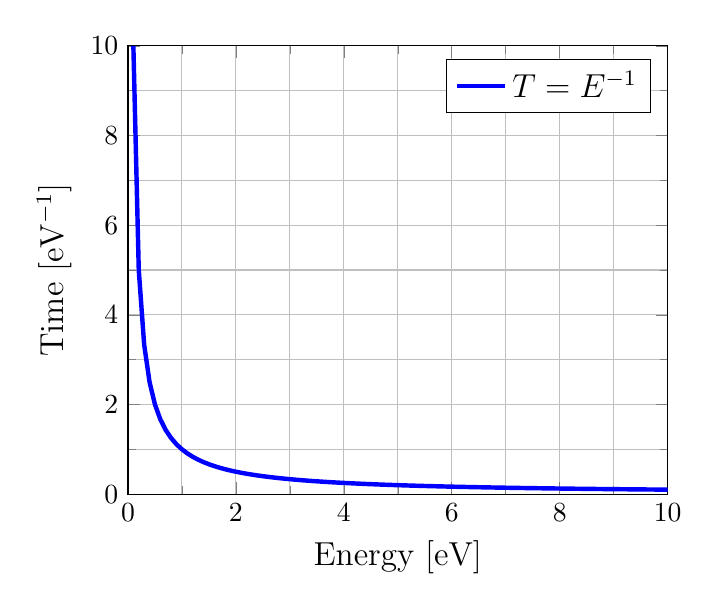
\begin{tikzpicture}
			\begin{axis}[
				xlabel={Energy [eV]},
				ylabel={Time [eV\(^{-1}\)]},
				xlabel style={font=\large},
				ylabel style={font=\large},
				tick label style={font=\normalsize},
				xmin=0, xmax=10,
				ymin=0, ymax=10,
				legend pos=north east,
				legend style={font=\large},
				grid=both,
				minor tick num=1
				]
				\addplot[blue, ultra thick, domain=0.1:10, samples=100] {1/x};
				\legend{\(T = E^{-1}\)}
			\end{axis}
		\end{tikzpicture}
		\caption{Energy-dependent time for photons.}
	\end{figure}
	
	\section{Experimental Verification}
	\begin{itemize}
		\item Frequency-dependent Bell tests.
	\end{itemize}
	
	\section{Physics Beyond the Speed of Light}
	\begin{equation}
		E^2 = (mc^2)^2 + (pc)^2 + \alpha_c p^4 c^2 / E_P^2
	\end{equation}
	
	\section{Conclusion}
	The dynamic mass of photons provides a novel view of nonlocality as an emergent phenomenon.
	
	\begin{thebibliography}{5}
		\bibitem{pascher1} Pascher, J. (2025). \textit{Time as an Emergent Property in Quantum Mechanics}.
		\bibitem{einstein} Einstein, A. (1905). \textit{On the Electrodynamics of Moving Bodies}. Annalen der Physik, 322(10), 891-921.
		\bibitem{planck} Planck, M. (1901). \textit{On the Law of Distribution of Energy in the Normal Spectrum}. Annalen der Physik, 309(3), 553-563.
		\bibitem{bell} Bell, J. S. (1964). \textit{On the Einstein Podolsky Rosen Paradox}. Physics, 1(3), 195-200.
		\bibitem{feynman} Feynman, R. P. (1985). \textit{QED: The Strange Theory of Light and Matter}. Princeton University Press.
	\end{thebibliography}
	
\end{document}